\documentclass{standalone}
\usepackage{tikz}
\usetikzlibrary{patterns, positioning}


\begin{document}
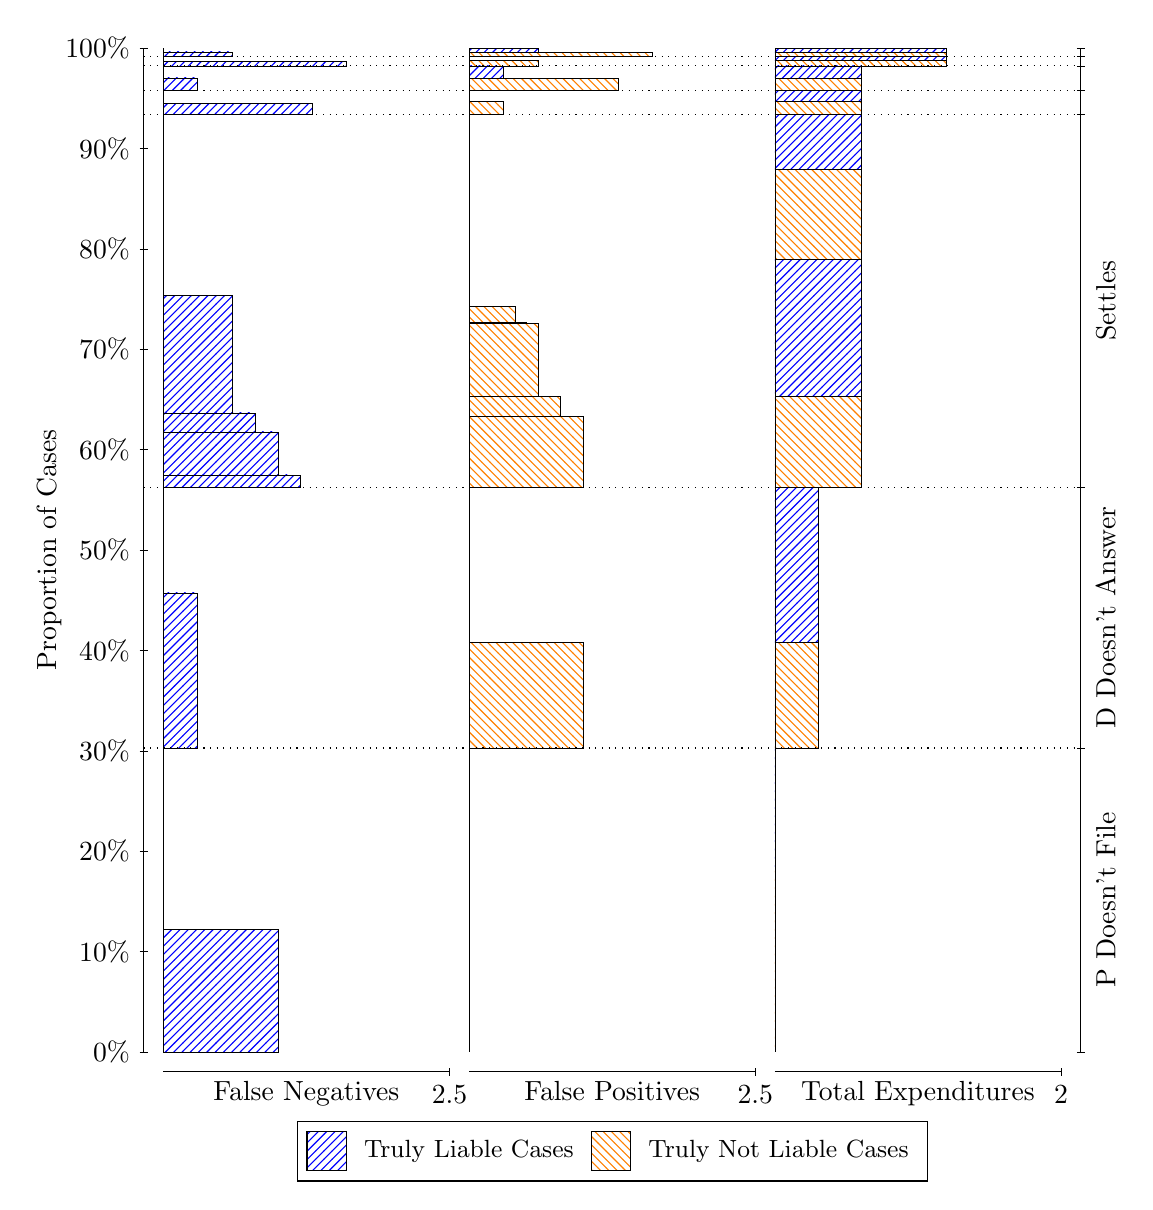
\begin{tikzpicture}
\draw[black, very thin] (1.5,1.75) -- (1.5,14.5);
\node[rotate=90, text=black, anchor=center] at (0.3, 8.125) {Proportion of Cases};
\draw[black, very thin] (1.45,1.75) -- (1.55,1.75);
\node[text=black, anchor=east] at (1.45, 1.75) {0\%};
\draw[black, very thin] (1.45,3.025) -- (1.55,3.025);
\node[text=black, anchor=east] at (1.45, 3.025) {10\%};
\draw[black, very thin] (1.45,4.3) -- (1.55,4.3);
\node[text=black, anchor=east] at (1.45, 4.3) {20\%};
\draw[black, very thin] (1.45,5.575) -- (1.55,5.575);
\node[text=black, anchor=east] at (1.45, 5.575) {30\%};
\draw[black, very thin] (1.45,6.85) -- (1.55,6.85);
\node[text=black, anchor=east] at (1.45, 6.85) {40\%};
\draw[black, very thin] (1.45,8.125) -- (1.55,8.125);
\node[text=black, anchor=east] at (1.45, 8.125) {50\%};
\draw[black, very thin] (1.45,9.4) -- (1.55,9.4);
\node[text=black, anchor=east] at (1.45, 9.4) {60\%};
\draw[black, very thin] (1.45,10.675) -- (1.55,10.675);
\node[text=black, anchor=east] at (1.45, 10.675) {70\%};
\draw[black, very thin] (1.45,11.95) -- (1.55,11.95);
\node[text=black, anchor=east] at (1.45, 11.95) {80\%};
\draw[black, very thin] (1.45,13.225) -- (1.55,13.225);
\node[text=black, anchor=east] at (1.45, 13.225) {90\%};
\draw[black, very thin] (1.45,14.5) -- (1.55,14.5);
\node[text=black, anchor=east] at (1.45, 14.5) {100\%};

\draw[black, very thin] (13.4,1.75) -- (13.4,14.5);
\draw[black, very thin] (13.35,1.75) -- (13.45,1.75);
\node[anchor=west] at (13.35, 1.75) {};
\draw[black, very thin] (13.35,5.6111) -- (13.45,5.6111);
\node[anchor=west] at (13.35, 5.6111) {};
\draw[black, very thin] (13.35,8.9235) -- (13.45,8.9235);
\node[anchor=west] at (13.35, 8.9235) {};
\draw[black, very thin] (13.35,13.657) -- (13.45,13.657);
\node[anchor=west] at (13.35, 13.657) {};
\draw[black, very thin] (13.35,13.961) -- (13.45,13.961);
\node[anchor=west] at (13.35, 13.961) {};
\draw[black, very thin] (13.35,14.274) -- (13.45,14.274);
\node[anchor=west] at (13.35, 14.274) {};
\draw[black, very thin] (13.35,14.393) -- (13.45,14.393);
\node[anchor=west] at (13.35, 14.393) {};
\draw[black, very thin] (13.35,14.5) -- (13.45,14.5);
\node[anchor=west] at (13.35, 14.5) {};

\draw[black, very thin, pattern color=blue, pattern=north east lines] (1.75,1.75) rectangle (3.2033,3.3101);
\draw[black, very thin, pattern color=orange, pattern=north west lines] (1.75,3.3101) rectangle (1.75,5.6111);
\draw[black, very thin, pattern color=blue, pattern=north east lines] (1.75,5.6111) rectangle (2.186,7.5794);
\draw[black, very thin, pattern color=orange, pattern=north west lines] (1.75,7.5794) rectangle (1.75,8.9235);
\draw[black, very thin, pattern color=blue, pattern=north east lines] (1.75,8.9235) rectangle (3.494,9.0711);
\draw[black, very thin, pattern color=blue, pattern=north east lines] (1.75,9.0711) rectangle (3.3487,9.0793);
\draw[black, very thin, pattern color=blue, pattern=north east lines] (1.75,9.0793) rectangle (3.2033,9.6238);
\draw[black, very thin, pattern color=blue, pattern=north east lines] (1.75,9.6238) rectangle (2.9127,9.8651);
\draw[black, very thin, pattern color=blue, pattern=north east lines] (1.75,9.8651) rectangle (2.622,11.357);
\draw[black, very thin, pattern color=orange, pattern=north west lines] (1.75,11.357) rectangle (1.75,13.657);
\draw[black, very thin, pattern color=blue, pattern=north east lines] (1.75,13.657) rectangle (3.6393,13.799);
\draw[black, very thin, pattern color=orange, pattern=north west lines] (1.75,13.799) rectangle (1.75,13.961);
\draw[black, very thin, pattern color=blue, pattern=north east lines] (1.75,13.961) rectangle (2.186,14.121);
\draw[black, very thin, pattern color=orange, pattern=north west lines] (1.75,14.121) rectangle (1.75,14.274);
\draw[black, very thin, pattern color=blue, pattern=north east lines] (1.75,14.274) rectangle (4.0753,14.326);
\draw[black, very thin, pattern color=orange, pattern=north west lines] (1.75,14.326) rectangle (1.75,14.393);
\draw[black, very thin, pattern color=blue, pattern=north east lines] (1.75,14.393) rectangle (2.622,14.452);
\draw[black, very thin, pattern color=orange, pattern=north west lines] (1.75,14.452) rectangle (1.75,14.5);
\draw[black, very thin, pattern color=orange, pattern=north west lines] (5.6333,1.75) rectangle (5.6333,4.051);
\draw[black, very thin, pattern color=blue, pattern=north east lines] (5.6333,4.051) rectangle (5.6333,5.6111);
\draw[black, very thin, pattern color=orange, pattern=north west lines] (5.6333,5.6111) rectangle (7.0867,6.9552);
\draw[black, very thin, pattern color=blue, pattern=north east lines] (5.6333,6.9552) rectangle (5.6333,8.9235);
\draw[black, very thin, pattern color=orange, pattern=north west lines] (5.6333,8.9235) rectangle (7.0867,9.8267);
\draw[black, very thin, pattern color=orange, pattern=north west lines] (5.6333,9.8267) rectangle (6.796,10.079);
\draw[black, very thin, pattern color=orange, pattern=north west lines] (5.6333,10.079) rectangle (6.5053,11);
\draw[black, very thin, pattern color=orange, pattern=north west lines] (5.6333,11) rectangle (6.36,11.011);
\draw[black, very thin, pattern color=orange, pattern=north west lines] (5.6333,11.011) rectangle (6.2147,11.223);
\draw[black, very thin, pattern color=blue, pattern=north east lines] (5.6333,11.223) rectangle (5.6333,13.657);
\draw[black, very thin, pattern color=orange, pattern=north west lines] (5.6333,13.657) rectangle (6.0693,13.819);
\draw[black, very thin, pattern color=blue, pattern=north east lines] (5.6333,13.819) rectangle (5.6333,13.961);
\draw[black, very thin, pattern color=orange, pattern=north west lines] (5.6333,13.961) rectangle (7.5227,14.114);
\draw[black, very thin, pattern color=blue, pattern=north east lines] (5.6333,14.114) rectangle (6.0693,14.274);
\draw[black, very thin, pattern color=orange, pattern=north west lines] (5.6333,14.274) rectangle (6.5053,14.341);
\draw[black, very thin, pattern color=blue, pattern=north east lines] (5.6333,14.341) rectangle (5.6333,14.393);
\draw[black, very thin, pattern color=orange, pattern=north west lines] (5.6333,14.393) rectangle (7.9587,14.441);
\draw[black, very thin, pattern color=blue, pattern=north east lines] (5.6333,14.441) rectangle (6.5053,14.5);
\draw[black, very thin, pattern color=orange, pattern=north west lines] (9.5167,1.75) rectangle (9.5167,4.051);
\draw[black, very thin, pattern color=blue, pattern=north east lines] (9.5167,4.051) rectangle (9.5167,5.6111);
\draw[black, very thin, pattern color=orange, pattern=north west lines] (9.5167,5.6111) rectangle (10.062,6.9552);
\draw[black, very thin, pattern color=blue, pattern=north east lines] (9.5167,6.9552) rectangle (10.062,8.9235);
\draw[black, very thin, pattern color=orange, pattern=north west lines] (9.5167,8.9235) rectangle (10.607,10.079);
\draw[black, very thin, pattern color=blue, pattern=north east lines] (9.5167,10.079) rectangle (10.607,11.812);
\draw[black, very thin, pattern color=orange, pattern=north west lines] (9.5167,11.812) rectangle (10.607,12.956);
\draw[black, very thin, pattern color=blue, pattern=north east lines] (9.5167,12.956) rectangle (10.607,13.657);
\draw[black, very thin, pattern color=orange, pattern=north west lines] (9.5167,13.657) rectangle (10.607,13.819);
\draw[black, very thin, pattern color=blue, pattern=north east lines] (9.5167,13.819) rectangle (10.607,13.961);
\draw[black, very thin, pattern color=orange, pattern=north west lines] (9.5167,13.961) rectangle (10.607,14.114);
\draw[black, very thin, pattern color=blue, pattern=north east lines] (9.5167,14.114) rectangle (10.607,14.274);
\draw[black, very thin, pattern color=orange, pattern=north west lines] (9.5167,14.274) rectangle (11.697,14.341);
\draw[black, very thin, pattern color=blue, pattern=north east lines] (9.5167,14.341) rectangle (11.697,14.393);
\draw[black, very thin, pattern color=orange, pattern=north west lines] (9.5167,14.393) rectangle (11.697,14.441);
\draw[black, very thin, pattern color=blue, pattern=north east lines] (9.5167,14.441) rectangle (11.697,14.5);
\draw[black, dotted] (1.5,5.6111) -- (13.4,5.6111);
\draw[black, dotted] (1.5,8.9235) -- (13.4,8.9235);
\draw[black, dotted] (1.5,13.657) -- (13.4,13.657);
\draw[black, dotted] (1.5,13.961) -- (13.4,13.961);
\draw[black, dotted] (1.5,14.274) -- (13.4,14.274);
\draw[black, dotted] (1.5,14.393) -- (13.4,14.393);
\draw[black, very thin] (1.75,1.5) -- (5.3833,1.5);
\node[text=black, anchor=north] at (3.5667, 1.5) {False Negatives};
\draw[black, very thin] (5.3833,1.45) -- (5.3833,1.55);
\node[text=black, anchor=north] at (5.3833, 1.45) {2.5};

\draw[black, very thin] (5.6333,1.5) -- (9.2667,1.5);
\node[text=black, anchor=north] at (7.45, 1.5) {False Positives};
\draw[black, very thin] (9.2667,1.45) -- (9.2667,1.55);
\node[text=black, anchor=north] at (9.2667, 1.45) {2.5};

\draw[black, very thin] (9.5167,1.5) -- (13.15,1.5);
\node[text=black, anchor=north] at (11.333, 1.5) {Total Expenditures};
\draw[black, very thin] (13.15,1.45) -- (13.15,1.55);
\node[text=black, anchor=north] at (13.15, 1.45) {2};

\node[text=black, centered, rotate=90] at (13.72, 3.6806) {P Doesn't File};
\node[text=black, centered, rotate=90] at (13.72, 7.2673) {D Doesn't Answer};
\node[text=black, centered, rotate=90] at (13.72, 11.29) {Settles};





\draw (7.449999999999999,1.5) node[draw=none] (baseCoordinate) {};
\begin{scope}[align=center]
        \matrix[scale=0.5, draw=black, below=0.5cm of baseCoordinate, nodes={draw}, column sep=0.1cm]{
            \node[rectangle, draw, minimum width=0.5cm, minimum height=0.5cm, pattern color=blue, pattern=north east lines] {}; &
            \node[draw=none, font=\small, text=black] (B) {Truly Liable Cases}; &
            \node[rectangle, draw, minimum width=0.5cm, minimum height=0.5cm, pattern color=orange, pattern=north west lines] {}; &
            \node[draw=none, font=\small, text=black] (B) {Truly Not Liable Cases}; \\
            };
\end{scope}

\end{tikzpicture}
\end{document}